\chapter{ACTUAL WORK} % Main chapter title
\label{ChapterActualWork} % For referencing the chapter elsewhere, use \ref{Chapter1} 


Upon completion of identifying \& formulating the research problem, and carrying out the necessary literature survey and review, the actual work on the project is taken-up. This chapter is dedicated to the actual work done by students. Hence, the chapter name and sub-chapter names are not fixed. It is left to the discretion of the students with appropriate guidance from their respective supervisors. However, one or more of the following aspects (as applicable) shall be covered in this chapter:
\begin{itemize}
	\item Methodology of the study or actual work (different from research methodology)
	\item Experimental and/or analytical work completed in the project
	\item Modeling, Analysis and Design
	\item Prototype and testing
\end{itemize}



\section{Methodology for the Study}\index{Methodology}

\section{Experimental and or Analytical Work Completed in the Project}

\section{Modeling, Analysis \& Design}

\section{Prototype \& testing}

\section*{Sample LaTeX Typesetting}


\paragraph*{Figure} Vector Graphics EPS Format [Figure \ref{fig:fcmc1}]
\begin{figure}[H]
	\begin{center}
		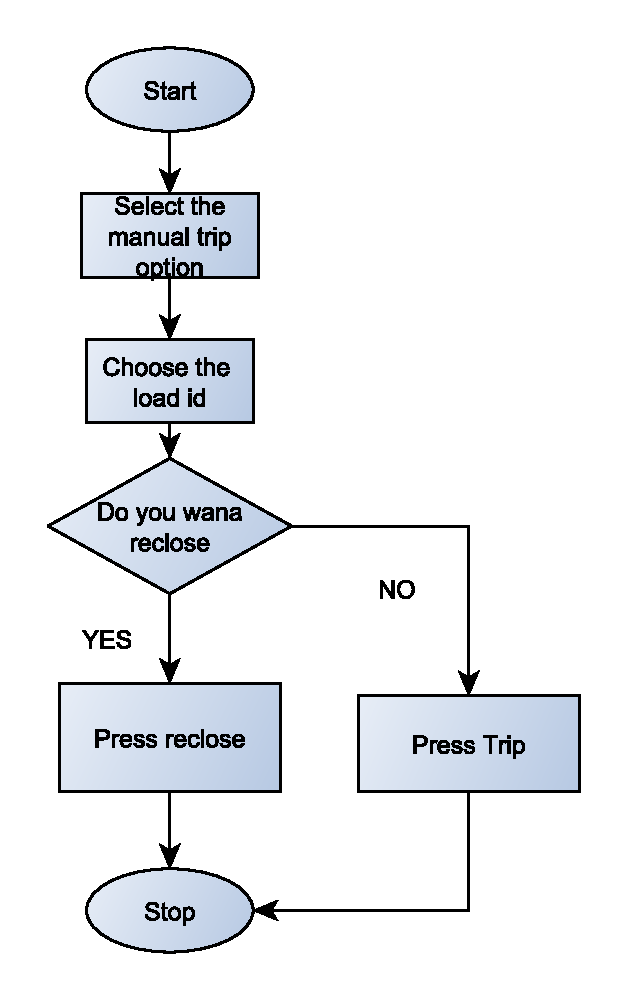
\includegraphics[scale=0.5]{Figures/manualtrip.eps}
		\caption{Flowchart of Manual Controller}
		\label{fig:fcmc1}
	\end{center}
\end{figure}


\paragraph*{Figure} JPEG/JPG Format [Figure \ref{fig:rb}]
\begin{figure}[h]
	\begin{center}
		\includegraphics[scale=0.3]{Figures/relay.jpg}
		\caption{Relay Board}
		\label{fig:rb}
	\end{center}
\end{figure}

\paragraph*{Table} Refer [Table \ref{tab:sm}]
\begin{table}[h]
	\centering
	\caption{Student Marks}
	\begin{tabular}{rr}
		\toprule
		Name  & Marks \\
		\midrule
		Ajay  & 10 \\
		Vinay & 20 \\
		\bottomrule
	\end{tabular}%
	\label{tab:sm}%
\end{table}%


\paragraph*{Cross References: Citation, Index, Reference, Equation reference}
This is the methodology for the entire project work which includes even the process of deciding on the project title, objectives
\index{Ojectives}, etc. This is mandatory for MTech and optional for BTech)\cite{abcdef}. The data is shown in Table \ref{tab:sm}. The equation shown in Equation \eqref{Eq:eq123}

\paragraph*{Inline Equation}
This is my equation.
$	f = ma \pm \alpha \Delta \left[ {\begin{array}{*{20}{c}}
	1 & \chi   \\
	{ - 1} & 0  \\
	\end{array}} \right] $
,which is appearing in between some text.

\paragraph*{Equation without Numbering} 
\begin{equation*}
	x = \frac{{ - b \pm \sqrt {{b^2} - 4ac} }}{{2a}}\
\end{equation*}

\paragraph*{Equation with Numbering} 
\begin{equation} \label{Eq:eq123}
\dot X = \left[ {\begin{array}{*{20}{c}}
	1 & p  \\
	2 & \alpha   \\
	\end{array}} \right]\left[ {\begin{array}{*{20}{c}}
	{{x_1}}  \\
	{{x_2}}  \\
	\end{array}} \right] + Bu\
\end{equation}



\paragraph*{Algorithm Format} 
\begin{algorithm}
	\caption{Addition of two 8 bit numbers}\label{alg:add8bit}
	\begin{algorithmic}[1]	
		\\ Start
		\\ Input a and b
		\\ c=a+b
		\\ Output c
		\\ stop
	\end{algorithmic}
\end{algorithm}


\paragraph*{Enumeration Format}
The following are the different flavor of Tex systems
\begin{enumerate}
	\item TeXLive TeX System
		\begin{enumerate}
			\item TeXLive for Windows
			\begin{enumerate}
				\item TeXLive
				\item ProTex
			\end{enumerate}
			\item MacTeX for Mac
		\end{enumerate}
	\item MikTeX TeX System
\end{enumerate}

\paragraph*{Bullets Format}
The following are the advantages of LaTeX,
\begin{itemize}
	\item {\LaTeX} is highly portable and free.
	\begin{itemize}
		\item Contribute to TUG
		\item Promote Free Softwares
	\end{itemize}
	\item Operating-system independent.
	\item Complex scientific documents can be created
	automatically.
	\item High quality math typesetting.
\end{itemize}

\paragraph*{Program Inclusion} Program file present in other directory can be embedded into the report.
\lstinputlisting{Files/code.asm}

\paragraph*{Verbatim Text} Include text as it is.
\\
The additional database schema is shown below which is used to store all the configuration and transaction data.
\begin{verbatim}
CREATE TABLE `controller_config` (
`load_id` int(11) NOT NULL,
`ct_constant` double DEFAULT NULL,
`pt_constant` double DEFAULT NULL,
`samples` int(11) DEFAULT NULL,
`delay` double DEFAULT NULL,
PRIMARY KEY (`load_id`)
) ENGINE=InnoDB DEFAULT CHARSET=utf8;
SELECT * FROM loadcontroller.load_details;
\end{verbatim} 


